% $Id: $
\documentclass[a4paper,11pt]{article}
\usepackage{a4wide}
\usepackage{enumerate}
\usepackage{amsmath,amsthm,amssymb}
\usepackage{amsfonts}
% The following makes latex use nicer postscript fonts.
\usepackage{times}
\usepackage{subcaption}
\usepackage{datatool}
\usepackage[utf8]{inputenc}
\usepackage{pdflscape}
\usepackage{longtable}
\usepackage{tocloft}
\usepackage{epigraph}

\usepackage[dutch]{babel}
\usepackage{tikz}
\usepackage[toc,page]{appendix}

%\usepackage[colorlinks,urlcolor=blue,linkcolor=blue]{hyperref}
\pagestyle{headings}
\newcommand{\upuparrow}{\mathrel{\reflectbox{\rotatebox[origin=c]{90}{$\twoheadrightarrow$}}}}
\newcommand{\downdownarrow}{\mathrel{\reflectbox{\rotatebox[origin=c]{90}{$\twoheadleftarrow$}}}}
\usepackage{vubtitlepage}
\usepackage{lmodern}
\usepackage{graphicx}

\usepackage[geometry]{ifsym}
%\usepackage[font=small,format=plain,labelfont=bf,up,textfont=it,up]{caption}
\renewcommand{\thefigure}{\thesection.\arabic{figure}}
\author{Filip Moons}
\title{Stagedossier}

\newtheorem{theorem}{Theorem}[section]
\newtheorem{lemma}[theorem]{Lemma}
\newtheorem{proposition}[theorem]{Proposition}
\newtheorem{conjecture}{Conjecture}
\newcommand{\tussen}[1]{\paragraph*{#1}\mbox{}\\}
\newtheorem{property}[theorem]{Property}
\newtheorem{definition}[theorem]{Definition}
\newtheorem{corollary}[theorem]{Corollary}
\newtheorem{remark}[theorem]{Remark}
\newtheorem{remarks}[theorem]{Remarks}
\newtheorem{notation}[theorem]{Notation}
\theoremstyle{definition}
\newtheorem{example}[theorem]{Example}
\newtheorem{examples}[theorem]{Examples}
 \usepackage[table,xcdraw]{xcolor}
\setcounter{tocdepth}{5}
\newcommand{\N}{{\mathbb N}}
\newcommand{\Z}{{\mathbb Z}}
\newcommand{\Q}{{\mathbb Q}}
\newcommand{\R}{{\mathbb R}}
\newcommand{\C}{{\mathbb C}}
\newcommand{\HQ}{{\mathbb H}}
\renewcommand{\P}{{\mathbb P}}
\newcommand{\E}{{\mathbb E}}
\newcommand{\cost}{\text{cost}}
\newcommand{\Nash}{\text{Nash}}
\newcommand{\Tau}{\mathrm{\tau}}
\newcommand{\nash}{\text{nash}}
\newcommand{\opt}{\text{opt}}
\newcommand{\LFP}{\text{LFP}}
\renewcommand{\int}{\text{int}}
\newcommand{\enquote}[1]{`#1'}
%\newenvironment{proof}{\noindent{\bf Bewijs.}}{{\hfill $ \ Box $}\vskip 4mm}

\promotortitle{Titularissen}
\promotor{Stagebegeleider Sophie Allein \\ Prof. Dr. B. Windels}
\advisors{}
\advisortitle{}
\addto\captionsenglish{\renewcommand*\abstractname{Abstract for non-mathematicians}}
\date{MEI 2006}
\faculty{Specifieke lerarenopleiding}
\advisortitle{}
\department{Wetenschappen \& Ingenieurswetenschappen}
\reason{Begeleide \& Zelfstandige oefenstage - Wiskunde}

\date{Januari 2014}


\begin{document}
% Then english TitlePage
\maketitlepage


\tableofcontents
\newpage
\section{Stagegegevens}
\subsection{Stageschool}
\textbf{MPIGO - Heemschool 1}

\textbf{Koninklijk Atheneum te Etterbeek}\\
\noindent 	E. Mesenlaan 2\\
\noindent  1040 Etterbeek\\

\\ \noindent Ik liep stage in het Koninlijk Atheneum van Etterbeek. Het KA Etterbeek is een Nederlandstalige school van het GO! Onderwijs van de Vlaamse Gemeenschap. 
De school bevindt zich in hartje Etterbeek, links van de Sint-Michielslaan, vlakbij metrostation Thieffry en tramhalte 
Boileau. \\

\noindent Het Gemeenschapsonderwijs (GO!) is een Vlaamse openbare instelling dat het officieel onderwijs organiseert in opdracht van de Vlaamse Gemeenschap. Het gemeenschapsonderwijs is een van de drie onderwijsnetten, naast het officieel 
gesubsidieerd en vrij gesubsidieerd onderwijs. In het gemeenschapsonderwijs hebben de ouders en de leerling de keuze voor de invulling van het vak levensbeschouwing: niet-confessionele zedenleer of katholieke, protestantse, anglicaanse, islamitische, Israëlitische of orthodoxe godsdienst. Ook vrijstelling van het vak levensbeschouwing is een mogelijkheid: vooral Jehova's getuigen en boeddhisten maken van deze mogelijkheid gebruik. Deze levensbeschouwelijke keuzevrijheid is het meest opvallende onderscheid tussen de scholen van Het Gemeenschapsonderwijs en de stedelijke, gemeentelijke, provinciale en VGC-scholen enerzijds, en vrije scholen van katholieke, niet-confessionele, protestantse of Joodse signatuur 
anderzijds.\\

\noindent Naast deze onderwijsvisie, zet de school zich ook in om volop de Brusselse 
context uit te spelen. Daarom zet ze zich in op de volledige ontplooiing van 
jongeren:  zij krijgen de kans om kennis te vergaren en sociale en creatieve vaardigheden te ontwikkelen. De multiculturele achtergrond, het engagement van het personeel, de educatieve projecten en de moderne infrastructuur zorgen voor een stimulerende leer- en leefomgeving waar iedere jongere zich thuis 
voelt.\\

\noindent De school kent een goede reputatie in Brussel, ze wordt gezien als één 
van de toonaangevende Nederlandstalige scholen in het Brusselse. Vooral op 
gebied van wetenschappen en wiskunde scoort de school zeer goed, onlangs werden ze zelf een STEM school of excellence (\emph{STEM = Science, Technology, Engeneering, Mathematics}).


\subsection{Klasgroepen}

\noindent\framebox(420, 82){ 
\parbox{400\unitlength}{\textbf{Opmerking}: De korte codes die ik aan elke klasgroep geef (5Wi8, 6Wi8 (Sophie), 6Wi8 (Lieselotte)) 
  zijn codes die ikzelf heb geïntroduceerd om de verschillende klasgroepen 
  waaraan ik stage heb gegeven gemakkelijk te onderscheiden. In realiteit schuilen 
  achter deze klasgroepen een bont allegaartje 5e of 6e jaars uit allerlei 
  richtingen (Latijn, Grieks, Wetenschappen,...), maar met 1 ding gemeen: ze 
  volgen allemaal 8uur wiskunde.}
}
\subsubsection{5Wi8}\label{5Wi8}
Het vijfde jaar met 8uur wiskunde bestaat uit 18 leerlingen die Latijn-Wiskunde, 
Grieks-Wiskunde, Economie-Wiskunde of Wetenschappen-Wiskunde volgen. De mentor is 
Lieselotte Monteyne.\\

\noindent Deze klas bevat een groepje jongens dat echt heel nieuwsgierig is naar wiskundige kennis. Deze heren durven zeker in de momenten met
 zelfstandig werk een spervuur van (vaak interessante) 
vragen stellen. Zij zitten ook altijd bij elkaar. Sommige vragen zijn zelf van danig hoog niveau, dat ik 
soms het antwoord moest voorbereiden tegen de volgende les.\\

\noindent Naast dat groepje 
nieuwsgierige jongens, zijn er ook nog andere groep, wat meer onzekere leerlingen. 
Deze leerlingenpopulatie koos vaak voor de 8 uur omdat het mooie 
toekomstperspectieven biedt, maar zij beseffen dat ze er hard voor zullen moeten 
werken om er te geraken. Het is deze groep die meteen panikeert als iets niet zo goed is 
uitgelegd geweest tijdens een stageles en die ook meteen klassikaal vragen 
afvuren om meer uitleg. Ook gezucht en luidop zeggen van `ik begrijp er niks 
van', is eigen aan deze groep. \\

\noindent In het algemeen een zeer aangename groep, met een tweedeling wat tot een divers 
publiek leidt. Het valt hier ook op dat het cognitief ontwikkelingsniveau tussen 
de leerlingen hier sterker verschilt dan in het 4e en 6e jaar: het 5e jaar is 
zowat het kruispunt tussen bijna uitgepuberde leerlingen en leerlingen die nog 
volop hun puberteit doormaken. In totaal gaf ik hier 14 uur les, grontendeels in de module `Begeleide oefenstage'.

\subsubsection{6Wi8 (Sophie)}\label{6Wi8a}
Het zesde jaar met 8uur wiskunde bestaat uit 17 leerlingen die allen 
Wetenschappen-Wiskunde studeren. De mentor in deze klas is tevens de stagebegeleider, Sophie Allein.\\

\noindent Naar het aanvoelen van mijn mentor, presteert deze klas nogal
matig om 8-uurs wiskunde te zijn. Ik moet bevestigen dat ik initieel ook hogere 
verwachtingen had van deze klasgroep, zeker omdat in het 5e jaar 8uur er zeer 
sterke leerlingen aanwezig waren. Toch was dit verruit de leukste klasgroep van 
allemaal.\\

\noindent Deze klasgroep was enorm aangenaam omdat ze zeer empathisch waren naar mij toe 
als stagiair. Als ze mij al wouden testen tijdens de zelfstandige oefenstage, dan was dat altijd plagend en nooit 
onrespectvol of beledigend bedoeld. Zij begrepen ook echt dat ik hier kwam om de `lerarenstiel' te leren 
en dat daar onvermijdelijk soms wat onzekerheid mee gepaard gaat. Sommigen 
wouden ook gelijkaardige richtingen gaan studeren volgend jaar als de mijne, 
waardoor sommige leerlingen me bijna met overdreven bewondering benaderden.\\

\noindent In totaal gaf ik hier 16 uur les, zowel in de module `Begeleide oefenstage' als 
in de module `Zelfstandige oefenstage'.

\subsubsection{6Wi8 (Lieselotte)}\label{6Wi8b}
De zesde jaar B met 8uur wiskunde bestaat uit 4 leerlingen die Latijn-Wiskunde, 
Economie-Wiskunde en Grieks-Wiskunde studeren. De mentor is hier opnieuw Lieselotte Monteyne. 
De reden waarom er twee 8uurs 
klassen zijn in het zesdejaar is simpelweg omdat teveel leerlingen zich 
inschreven. Deze 4 leerlingen volgen daarom les bij het zesde jaar met 6uur 
wiskunde en krijgen daarbovenop nog 2 uitbreidingsuren. Ik heb hen 4 
uitbreidingsuren gegeven rond computerwetenschappen, allen in de module 
`Zelfstandige oefenstage.'\\

\noindent De klasgroep was heel klein en daardoor ook vrij passief. 1 van de 4 leerlingen 
doet aan topsport en moest daarom niet alle lessen meevolgen. Deze leerling was 
ook extreem verlegen.\\

\noindent Al bij al een fijne klasgroep, al vermoed ik dat hun passiviteit deels te wijten 
was aan het feit dat ze van mij uitsluitend uitbreidingsleerstof kregen die 
sowieso nooit geëvalueerd zou worden. Ze kenden mij niet vooraf van andere 
lessen.

\subsubsection{4SW}\label{4SW}
Het vierde jaar Sport-Wetenschappen is een klas met 19 leerlingen, waarvan 17 
jongens. De mentor is hier David Maquenne.\\

\noindent Deze klas kreeg 6 uur les van mij, op het einde van de module `Zelfstandige 
oefenstage'. Vooraf ben ik hen gaan observeren (heb ik in elke klas gedaan, \emph{cfr. Stageplanning}) 
en het viel me op dat het niet zo makkelijk is deze klas in het gareel te houden. Papiertjes werden in het rond gegooigd, er werd voortdurend gepraat, 
leerlingen waren met hun gsm's bezig, er werd geprutst met het aanwezige materiaal in de 
klas,... De mentor zelf bleef er heel kalm bij, maar ik zat na die observaties met 
heelwat vragen. Ik ben namelijk niet zo kalm aangelegd als mijn mentor, mijn 
irritatiegrens ligt een pak lager als bij hem. \\

\noindent Uiteindelijk had ik bedacht om overal consequent op in te grijpen en een beetje 
arrogant uit de hoek te komen als hulpmiddelen voor het klasmanagement. Tot op 
zekere hoogte wierp dat zijn vruchten af. Toch was de tijd te beperkt om het effect van 
deze hulpmiddelen langdurig te verzilveren: de klas bleef hoe dan ook vrij rumoerig. \\


\subsection{Stageplanning}
\begin{center}
  \framebox{Alle stageweken voor de herfstvakantie behoren tot de module `Begeleide oefenstage'.}
\end{center}
\subsubsection{Week 1: 22-26 september}
\newcommand{\klasvijf}[2]{\item\textcolor{ocre}{\textbf{5Wi8}}: #1 - #2}
\newcommand{\klaszes}[2]{\item\textcolor{ocre}{\textbf{6Wi8 (Sophie)}}: #1 - #2}
\newcommand{\klasklein}[2]{\item\textcolor{ocre}{\textbf{6Wi8 (Lieselotte)}}: #1 - #2}
\newcommand{\kutklas}[2]{\item\textcolor{ocre}{\textbf{4SW}}: #1 - #2}
 \paragraph*{Woensdag 24 september}
\begin{itemize}
   \klaszes{08u10-09u00 (1e lesuur)}{Observatie}
   \klaszes{09u00-09u50 (2e lesuur)}{Observatie}
  \end{itemize}
  
\paragraph*{Donderdag 25 september}
\begin{itemize}
   \klasvijf{13u30-14u20 (7e lesuur)}{Observatie}
   \klasvijf{15u20-16u10 (9e lesuur)}{Observatie}
  \end{itemize}

\subsubsection{Week 2: 29 september - 3 oktober}
\paragraph*{Maandag 29 september}
\begin{itemize}
      \klaszes{09u00-09u50 (2e lesuur)}{Combinatoriek - keuzes met herhaling}
  \end{itemize}
  \paragraph*{Dinsdag 30 september}
\begin{itemize}
      \klaszes{08u10-09u00 (1e lesuur)}{Combinatoriek - keuzes met herhaling}
   \klaszes{09u00-09u50 (2e lesuur)}{Combinatoriek - keuzes met herhaling}
     \end{itemize}
\paragraph*{Donderdag 2 oktober}
\begin{itemize}
   \klasvijf{13u30-14u20 (7e lesuur)}{Combinatoriek - inleiding}
     \end{itemize}
\paragraph*{Vrijdag 3 oktober}
\begin{itemize}
   \klasvijf{09u00-09u50 (2e lesuur)}{Combinatoriek - keuzes zonder herhaling}
  
  \end{itemize}
  
 \subsubsection{Week 3: 6-10 oktober}

\paragraph*{Dinsdag 7 oktober}
\begin{itemize}
      \klaszes{08u10-09u00 (1e lesuur)}{Combinatoriek - keuzes met herhaling}
   \klaszes{09u00-09u50 (2e lesuur)}{Combinatoriek - keuzes met herhaling}
   \klasvijf{11u00-11u50 (4e lesuur)}{Combinatoriek - keuzes zonder herhaling}
     \end{itemize}
 \paragraph*{Donderdag 9 oktober}
 \begin{itemize}
     \klaszes{09u00-09u50 (2e lesuur)}{Combinatoriek - keuzes met herhaling}
     \klasvijf{13u30-14u20 (7e lesuur)}{Combinatoriek - keuzes zonder herhaling}
         \klasvijf{15u20-16u10 (8e lesuur)}{Combinatoriek - keuzes zonder herhaling}
     \end{itemize}
 \subsubsection{Week 4: 13-17 oktober}

\paragraph*{Dinsdag 7 oktober}
\begin{itemize}
      \klaszes{08u10-09u00 (1e lesuur)}{Combinatoriek - Driehoek van Pascal}
   \klaszes{09u00-09u50 (2e lesuur)}{Combinatoriek - Binomium van Newton}
   \klasvijf{11u00-11u50 (4e lesuur)}{Combinatoriek - keuzes met herhaling}
     \end{itemize}
 \paragraph*{Donderdag 9 oktober}
 \begin{itemize}
     \klaszes{09u00-09u50 (2e lesuur)}{Combinatoriek - Toets}
     \klasvijf{13u30-14u20 (7e lesuur)}{Combinatoriek - keuzes met herhaling}
         \klasvijf{15u20-16u10 (8e lesuur)}{Combinatoriek - keuzes met herhaling}
          \end{itemize}
   
  \subsubsection{Week 5: 20-24 oktober}

\paragraph*{Dinsdag 7 oktober}
\begin{itemize}
      \klaszes{08u10-09u00 (1e lesuur)}{Inleiding tot de computerwetenschappen (Uitbreidingsleerstof)}
   \klaszes{09u00-09u50 (2e lesuur)}{lnleiding tot de computerwetenschappen (Uitbreidingsleerstof)}
     \end{itemize}
 \paragraph*{Donderdag 9 oktober}
 \begin{itemize}
     \klaszes{09u00-09u50 (2e lesuur)}{Inleiding tot de computerwetenschappen (Uitbreidingsleerstof)}
     \klasklein{09u50-10u40 (3e lesuur)}{Observatie}
     \klasvijf{13u30-14u20 (7e lesuur)}{Combinatoriek - Toets}
         \klasvijf{15u20-16u10 (8e lesuur)}{Combinatoriek - keuzes met herhaling}
    \end{itemize}
   
  \subsubsection{Week 6: 27-31 oktober}
Geen les, herfstvakantie

  \subsubsection{Week 7: 3-7 november}

\begin{center}
  \framebox{Na de herfstvakantie behoren alle lessen tot de module `Zelfstandige oefenstage.'}
\end{center}

\paragraph*{Maandag 3 november}
\begin{itemize}
      \klaszes{09u00-09u50 (2e lesuur)}{Kegelsneden: Inleiding}
      \klaszes{12u40-13u30 (6e lesuur)}{Kegelsneden: De Parabool}
  \end{itemize}
  
 \paragraph*{Dinsdag 4 november}
\begin{itemize}
       \klaszes{08u10-09u00 (1e lesuur)}{Kegelsneden: De Parabool}
      \klaszes{09u00-09u50 (2e lesuur)}{Kegelsneden: De Parabool}
  \end{itemize}
  
   \paragraph*{Woensdag 5 november}
\begin{itemize}
       \klasklein{11u50-12u40 (5e lesuur)}{Inleiding tot de computerwetenschappen (Uitbreidingsleerstof)}
  \end{itemize}
   \paragraph*{Donderdag 6 november}
\begin{itemize}
  \klasklein{09u50-10u40 (3e lesuur)}{Inleiding tot de computerwetenschappen (Uitbreidingsleerstof)}
       \kutklas{11u00-11u50 (4e lesuur)}{Observatie}
  \end{itemize}
     \paragraph*{Vrijdag 7 november}
\begin{itemize}
       \kutklas{13u30-14u20 (7e lesuur)}{Observatie}
  \end{itemize}
  
  
    \subsubsection{Week 8: 10-14 november}

\paragraph*{Maandag 10 november}
\begin{itemize}
      \klaszes{09u00-09u50 (2e lesuur)}{Kegelsneden: De Parabool}
      \klaszes{12u40-13u30 (6e lesuur)}{Kegelsneden: De Parabool}
  \end{itemize}
  
  \paragraph*{Dinsdag 11 november}
Feestdag

\paragraph*{Woensdag 12 november}
\begin{itemize}
      \klaszes{09u00-09u50 (2e lesuur)}{Kegelsneden: De Parabool}
   \klasklein{11u50-12u40 (5e lesuur)}{Inleiding tot de computerwetenschappen (Uitbreidingsleerstof)}

  \end{itemize}
  
   \paragraph*{Donderdag 13 november}
\begin{itemize}
        \klaszes{09u00-09u50 (2e lesuur)}{Kegelsneden: De Parabool}

  \klasklein{09u50-10u40 (3e lesuur)}{Inleiding tot de computerwetenschappen (Uitbreidingsleerstof)}
       \kutklas{11u00-11u50 (4e lesuur)}{Georiënteerde hoeken}
  \end{itemize}
  
       \paragraph*{Vrijdag 14 november}
\begin{itemize}
       \kutklas{13u30-14u20 (7e lesuur)}{Georiënteerde hoeken}
  \end{itemize}
  
      \subsubsection{Week 9: 17-21 november}
  \paragraph*{Donderdag 20 november}
\begin{itemize}
  \kutklas{09u50-10u40 (3e lesuur)}{Georiënteerde hoeken}
       \kutklas{11u00-11u50 (4e lesuur)}{Georiënteerde hoeken}
  \end{itemize}
  \paragraph*{Vrijdag 14 november}
\begin{itemize}
       \kutklas{13u30-14u20 (7e lesuur)}{Georiënteerde hoeken}
  \end{itemize}


\newpage
\section{Algemene reflectie}
De begeleide- \& zelfstandige oefenstage werd pas begin september geregeld. Na 
het aanvragen en bekomen van enkele vrijstellingen op basis van een jaar 
lerarenopleiding aan de hogeschool, was een regulier stagetraject ineens pakken 
interessanter geworden dan de geplande LIO-baan in het schooljaar 2015-2016. 
Enkele toelatingen van vakgroepvoorzitters en enkele herplanningen later, maakten 
de weg vrij voor nieuw stage-avontuur. De stagebegeleidster, mevrouw Allein, 
stelde voor om de stage op haar school te doen, dat maakte het voor alle 
partijen makkelijker. Vermits enkele weken nadien de stage al zou beginnen, ging 
uiteraard graag op dit aanbod in.\\

\noindent De eerste stageweek was al meteen goedgevuld: 8 uur les te geven en 2 
uurtjes observatie. Wat meteen opviel tijdens de eerste stageles: de inhoud van 
de leerstof bepaalt enorm het lesverloop. Ik had immers al stage gelopen in mijn 
jaar lerarenopleiding aan de hogeschool, maar een lesuur vullen met de 
eigenschappen van vierkanten is iets helemaal anders dan de geheimen van de 
combinatoriek verklaren. Ook de nood aan structuur die leerlingen hadden was 
overweldigend: na 5 jaar universiteit ben je dat voorgekauw immers verleerd. Het 
overbrengen van bepaalde leerstof die voor jezelf zo logisch is is ook geen 
evidentie: als beginneling is het niet altijd goed in te schatten welke 
instructie de leerlingen nodig hebben om nieuwe concepten te vatten.\\

\noindent Al bij al waren die eerste weken best confronterend. Ik die met mijn 
ervaring uit het regentaat nog dacht dat de stage van een leien dakje zou 
verlopen, werd geconfronteerd met onverwachte moeilijkheden. Na enkele lessen 
begon ik daarom, naast de lesvoorbereidingen, ook met bordschema's te maken. Dat 
krikte de structuur op het bord en bijgevolg de hele les op. Ook begon ik meer 
na te denken over mogelijke vragen van leerlingen, het was immers een paar keer 
voorgevallen dat ik overweldigd was door vragen waar ik niet meteen een antwoord 
op kon verzinnen. \\

\noindent Naarmate de tijd vorderde, werd ook het contact met de leerlingen 
beter om beter. Allerlei vragen kwamen: wie bent u eigenlijk? Wat studeer je? Ik 
zou volgend jaar die richting willen doen, zou me dat lukken denk je? ... Vooral 
de vraagmomenten over de middag waren toenaderingsmomenten voor beide partijen. 
Vooral het feit dat ikzelf nog piepjong ben en nog met beide voeten op de 
universiteit zit, maakte mij een gewillig doelwit voor al hun vragen. \\

\noindent Tijdens de stagelessen zelf probeerde ik zoveel mogelijk te werken aan 
mijn structuur, heldere uitleg en bordschema's. Waar ik in het begin van de 
stage nog vrij traditionele werkvormen hanteerde, durfde ik ook meer en meer 
iets uitdagender uit de hoek komen. Zo kwam ik met een spelvorm voor het 
uitleggen van sorteeralgoritmes en met hoekenwerk rond toepassingen van de 
parabool.\\

\noindent In de lessen bij het 4e jaar waren er een beetje problemen met 
klasmanagement, die ik van meters ver zag aankomen. Tijdens mijn observatielesuur 
was het er ook zeer onrustig bij de mentor. Ik heb toen contact opgenomen met 
professor Windels om raad te vragen en ik heb zogoed als mogelijk mij 
gepresenteerd als leerkracht. Professor Windels had me echter gewaarschuwd dat 
het nagenoeg onmogelijk zou zijn om het op gebied van klasmanagement beter te 
doen de de oorspronkelijke leerkracht, waardoor ik hier ook niet te lang bij 
stil wil staan. Didactisch zaten deze lessen wel vrij goed ineen. Ik denk 
persoonlijk niet dat ik later veel problemen zal hebben met klasmanagement, daar 
ik die in de overige klasgroepen maar ook in vroegere ervaringen nooit gehad 
heb. Duidelijke afspraken met de leerlingen maken en die consequent bewaken is 
samen met een scheut humor en menselijkheid immers voldoende om de meeste 
problemen op dat gebied op te lossen. Een onrustige klas veranderen op 6 uren tijd, is echter wel onmogelijk.\\ 

\noindent Al bij al is de stage enorm goed meegevallen. Bordschrift, structuur 
en inleven in de leefwereld van de leerling blijven prioriteiten om aan te 
werken als ik in september 2015 zelf voor de klas sta. Er zijn uiteraard nog 
andere `zwaktes', maar het lijkt me niet verstandig aan alles in 1 keer te 
willen werken. Als ik op deze 3 domeinen fundamentele professionelere 
verbetering boek, dan volgt de rest vanzelf wel. Het kan zeker niet de bedoeling 
zijn om met jezelf als beginnend leerkracht op alle fronten ineens de strijd aan te 
gaan, er moet ook genoten kunnen worden. Dat genot is de basis voor een loopbaan 
in het onderwijs als gemotiveerde leerkracht. Ik kijk alvast uit naar september 
2015, want Brussel heeft er dan een wiskundeleerkracht bij.
\newpage
\section{Extra opdrachten Zelfstandige oefenstage}
\subsection{Opdracht 1: Periode- \& vorderingsplan}
Noot vooraf: ik heb maar liefst in 4 verschillende klasgroepen gestaan tijdens 
de zelfstandige oefenstage en om praktische redenen omvatte de zelfstandige 
oefenstage slechts 16 lesuren, de begeleide oefenstage 24 lesuren. In elke klas stond ik hoogstens 6 uur. Een echt 
`periodeplan' maken is hier dus ietwat overdreven gezien het zeer beperkt aantal lesuren per klasgroep.
 In de 4SW stond ik 6uur, in 
de 6Wi8 bij mevrouw S. Allein stond ik nogmaals 4 uur. Ik neem specifiek deze 
klassen om een zeer bescheiden periodeplanning te presenteren en de vorderingen 
hierop aan te geven. In de klassen bij mentor L. Monteyne gaf ik ofwel slechts 2 
uren les (5Wi8) ofwel gaf ik 4u uitbreidingsleerstof rond computerwetenschappen (6Wi8) 
waarbij er geen link kan gelegd worden met het respectievelijke jaarplan. 
Daardoor focus ik mij voor deze opdracht dus uitsluitend op de 4SW en 6Wi8 
(Sophie).
\subsubsection{6Wi8}
\paragraph{Jaarplan van de mentor}
In figuur \ref{jaar1} ziet u het deel uit het jaarplan van de mentor dat 
betrekking heeft op de gegeven stagelessen tijdens de zelfstandige oefenstage. 
De mentor voorziet slechts 1,5 uur voor de hele thematiek rond kegelsneden en 
dit op het einde van het schooljaar. Dit is duidelijk een onderwerp waar weinig 
belang wordt aan gehecht en dat allicht wegvalt indien andere prioritaire 
leerstof nog niet aanbod kwam. Het leerplan lijkt de mentor hierin te steun, deze zijn immers ook veel minder
ambitieus dan de leerstof in het gebruikte handboek:
\begin{itemize}
  \item kennen de ruimtelijke interpretatie van kegelsneden als snijding van een kegel met
een vlak;
\item kennen de meetkundige definities van parabool, ellips en hyperbool, alsook de bijhorende terminologie en notaties;
\item kunnen de cartesische vergelijking opstellen van parabool (betrokken op as en
topraaklijn), ellips en hyperbool (betrokken op de assen);
\item kunnen het stelsel parametervergelijkingen van een ellips opstellen;
\item kunnen in een punt van de bestudeerde kegelsneden de cartesische vergelijking van
de raaklijn en de normaal opstellen, en deze raaklijn en normaal meetkundig construeren;
\item kunnen toepassingen en voorbeelden van kegelsneden in andere disciplines.
\end{itemize}
Toch lijkt anderhalf uur wel erg bescheiden om alle doelstellingen te kunnen 
realiseren. 

\begin{figure}[h]
 \centering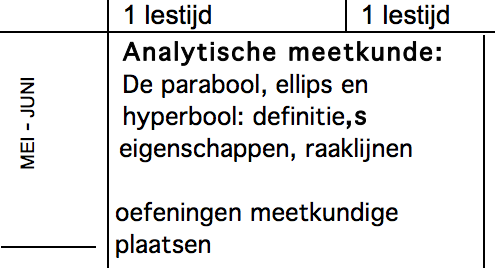
\includegraphics[scale=0.6]{jaarplan2.png} 
\caption{Jaarplan van de mentor 6Wi8 m.b.t. gegeven stagelessen.}}\label{jaar1}
\end{figure}
\paragraph{Eigen periode-\& vorderingsplan}
Vermits het jaarplan van de mentor voor deze leerstof en periode toch vrij 
bescheiden is, presenteer ik hieronder een uitgebreider periode- \& 
vorderingsplan. Het valt op dat de laatste leerinhoud/leerdoelstelling niet 
gerealiseerd werd. Dit komt omdat er vertraging is opgelopen in de voorgaande 
lesuren. Een werkvorm met hoekenwerk rond de toepassingen van de hoofdstelling 
van de parabool was begroot op 25 minuten in de lesvoorbereiding (zie bijlage 
4.2.2.2.), maar heeft uiteindelijk een volledig lesuur in beslag genomen. De 
leerlingen waren iets te gemotiveerd bezig met alles waardoor ik niet 
vroegtijdig wou afbreken. De oefeningen werden daardoor digitaal doorgestuurd en 
niet meer klassikaal behandeld.

\begin{table}[h]
\begin{tabular}{|l|l|l|l|}
\hline

\textbf{\begin{tabular}[c]{@{}l@{}}Leerplan-\\ doelstellingen\end{tabular}} & \textbf{Leerinhoud}                                                                                                                                                        & \textbf{\begin{tabular}[c]{@{}l@{}}Aantal\\lestijden\end{tabular}} & \textbf{Vordering} \\ \hline
5.2                                                                                                & \begin{tabular}[c]{@{}l@{}}De leerlingen kunnen de begrippen \\ kegelsneden en meetkundige plaats uitleggen.\end{tabular}                                                                          & 1                                                & Geslaagd                                  \\ \hline
5.2                                                                                                & \begin{tabular}[c]{@{}l@{}}De leerlingen kunnen de parabool \\ uitdrukken als meetkundige plaats, als \\ parametervergelijking en kunnen de \\ parametervergelijking ook onderzoeken.\end{tabular} & 1                                                & Geslaagd                                  \\ \hline
Uitbreiding                                                                                        & \begin{tabular}[c]{@{}l@{}}De leerlingen kunnen de hoofd-eigenschap \\ van de parabool opzeggen, bewijzen en \\ toepassingen uit het dagelijkse leven van \\ opnoemen.\end{tabular}                & 2                                                & Geslaagd                                  \\ \hline
5.2.                                                                                               & \begin{tabular}[c]{@{}l@{}}De leerlingen kunnen allerlei soorten \\ oefeningen oplossen met de geziene theorie\\ rond parabolen.\end{tabular}                                                      & 1                                                & Niet gelukt                               \\ \hline
\end{tabular}
\end{table}

\subsubsection{4SW}
Het deel in het jaarplan rond de gegeven stagelessen in 4SW vindt u terug in 
figuur \ref{jaar2}. Dit jaarplan is erg uitgebreid en accuraat met mijn eigen 
periodeplanning. Ik had inderdaad 6 lesuren en alle onderdelen die in het 
jaarplan stonden zijn volgens de begrote lesuren effectief kunnen uitgevoerd 
worden. De betreffende lesvoorbereidingen vindt in de bijlagen 4.2.1.
\begin{figure}[h!]
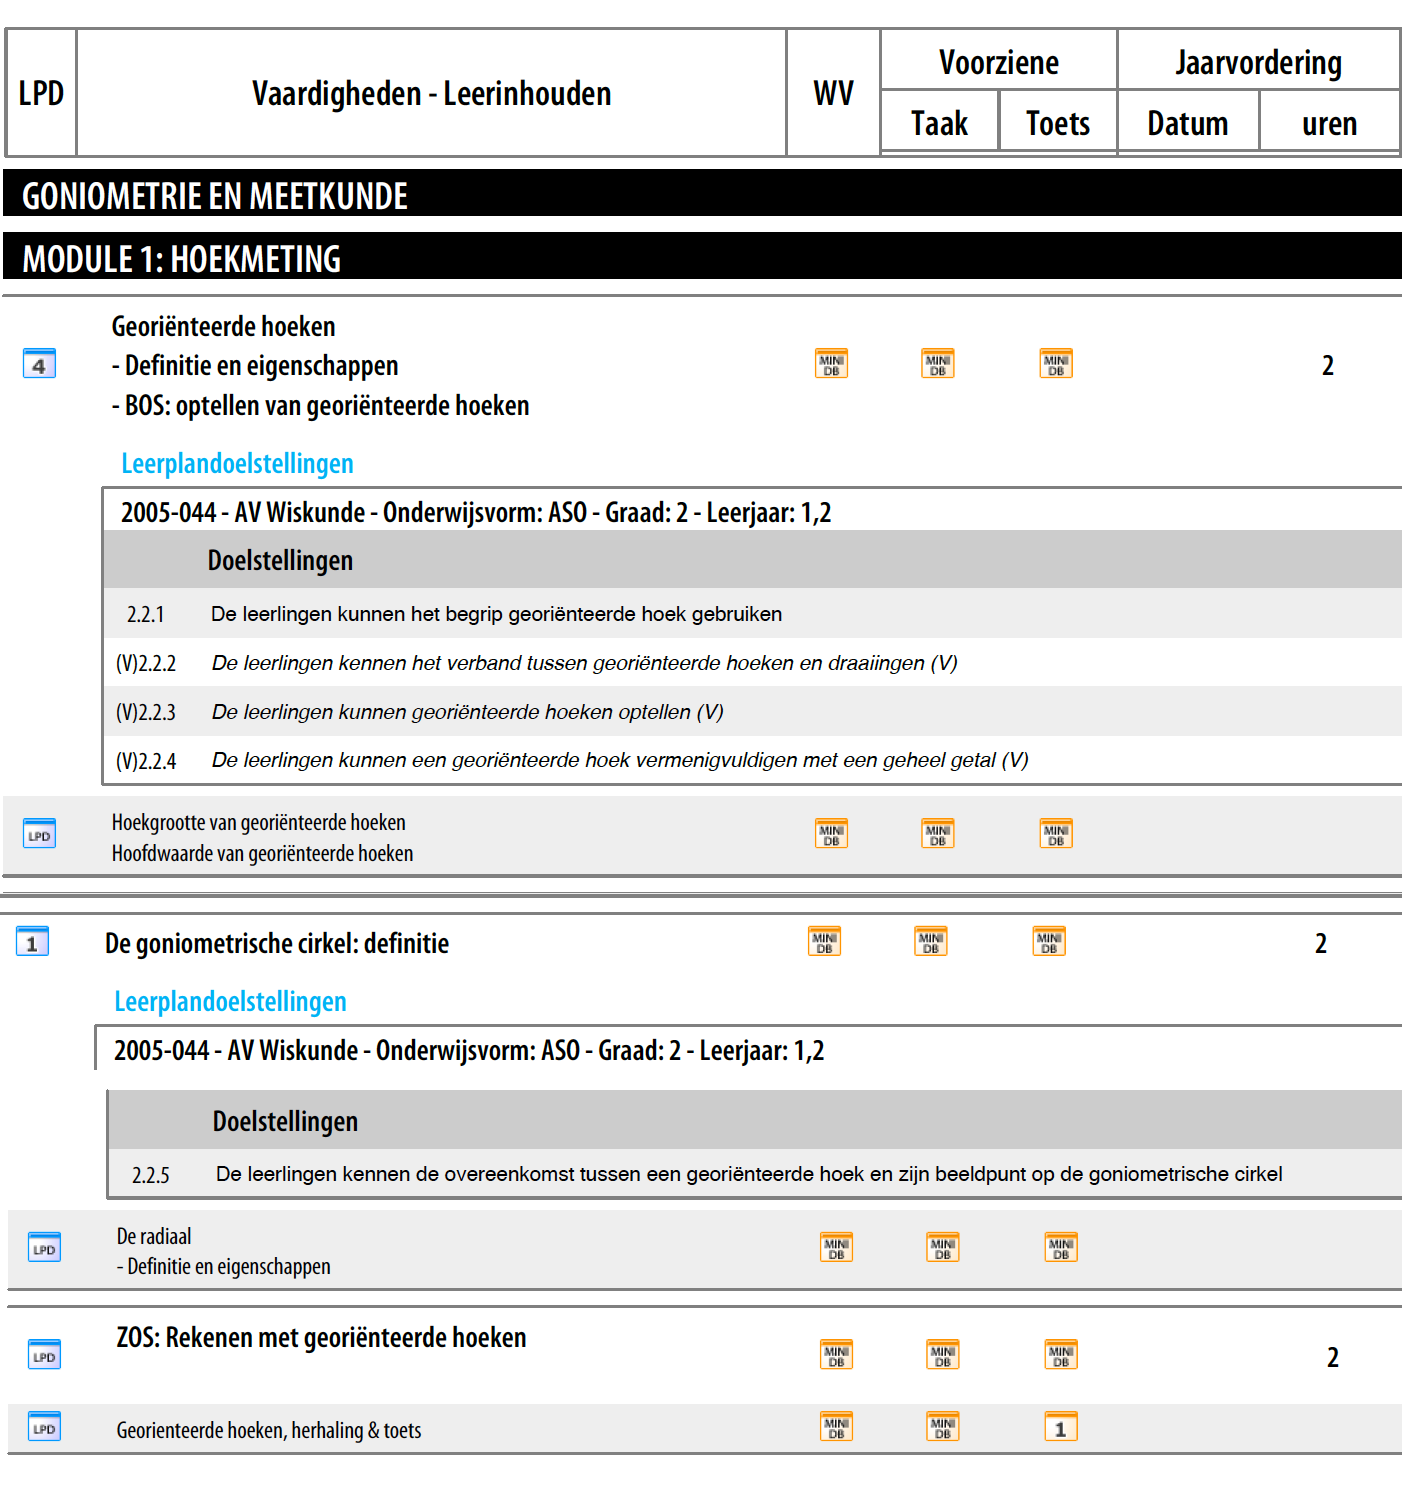
\includegraphics[scale=0.6]{jaarplan.png}
\caption{Jaarplan van de mentor 4SW m.b.t. gegeven stagelessen.}}\label{jaar2}
\end{figure}
\newpage
\subsection{Opdracht 2: Evaluatie van de leerlingen}
Vermits ik zoals reeds opgemerkt in opdracht 1 slechts heel beperkte lessenreeksjes gegeven heb tijdens de 
zelfstandige oefenstage, gaat deze toets over leerstof die behandeld werd 
tijdens de stagelessen in de 5Wi8 tijdens de begeleide oefenstage. De toets zelf 
vond wel plaats tijdens de zelfstandige oefenstage. De toets vind je terug in 
bijlage 4.2.3.3. De toets is een herhalingsoverhoring rond combinatoriek - keuzes met én zonder herhaling.
Hierbij werden volgende visie, regels- en afspraken gehanteerd,
in samenspraak met de mentor:
\begin{itemize}
  \item Uitsluitend ondervragen van oefeningen, geen theorie. Ook de notaties 
  die in de les werden ingevoerd rond (herhalings)variaties, 
  (herhalings)permutaties en (herhalings)combinaties moesten niet verplicht in 
  de antwoorden gezet worden door de leerlingen. Het was uiteraard wel een goed 
  idee omdat wel te doen, want dit levert punten op bij een fout eindresultaat.
  \item De toets zelf ondervraagt zowel keuzes mét als zonder herhaling. 
  Heel bewust zijn er meer oefeningen rond keuzes met herhaling, vermits daar 
  nog geen overhoring over was. De oefeningen rond keuzes zonder herhaling zijn 
  verwerkt in een grote slotvraag.
  \item Bij de verbetering is het belangrijk op voorhand een ingevulde toets te 
 maken en een puntenverdeling voor elke oefening vast te leggen. Indien leerlingen onverwachte antwoorden
geven, moeten zij een bepaald punt krijgen en moet dit ook op mijn verbetersleutel genoteerd worden. 
Zo kan bij herhaling van deze onverwachte antwoorden hetzelfde cijfer aan een leerling worden toegekend.
De mentor hamert hier echt op om zo een zo eerlijk mogelijke quotatie voor de 
leerlingen onderling te garanderen. Zij vroeg ook naar mijn verbetersleutel toen ik 
de toetsen teruggaf.
\item Qua punten kwam ik tot dezelfde resultaten als bij de mentor: 3 leerlingen 
waren gebuisd (wat een normaal aantal is volgens haar) en de leerlingen die zwak 
scoorden, hebben al vaker zwak gescoord.
\item Er werd ook een inhaaltoets opgesteld voor een zieke leerling en een taak (bijlage 4.2.3.4) 
voor leerlingen die extra willen oefenen of een tekort haalden.
\end{itemize}


\subsection{Opdracht 3: Neerslag gesprekken met de mentor}
Ik heb niet echt structureel telkens ik een gesprek had met de mentor 
opgeschreven wat zij/hij vertelde, enkel de belangrijke kernboodschappen. De 
lijst ik hier steeds op per mentor.
\subsubsection{Sophie Allein}
\begin{itemize}
  \item Geeft me vooral mee dat ik hoofd- \& bijzaak goed van elkaar dien te 
  onderscheiden. Soms is het belangrijk bepaalde details niet mee te geven 
  teneinde het grote verhaal niet te laten verloren gaan.
  \item Geeft mee dat er nog iets meer structuur mag aangebracht worden en het 
  tempo soms wat hoger mag liggen.
  \item Geeft mee dat het bordschrift een aandachtspunt blijft, maar dat het wel al sterk verbeterd is.
  \item Geeft mee dat er nooit, al is het goedbedoeld, spottend mag gedaan worden over namen. Dit kan kwetsend overkomen.
  \item Geeft mee dat bewijzen best niet volledig uitgeschreven op bord komen indien ze te lang zijn. Leerlingen hebben
  een handboek en hoeven dus ook niet altijd alles over te pennen. 
  \item Hamert op een correct gebruik van het Nederlands en schuwt de `ge'-vorm.
\end{itemize}
\subsubsection{Lieselotte Monteyne}
\begin{itemize}
  \item Vind dat ik enorm gegroeid ben tijdens de stageperiode: van 
  ongestructureerd en warrig naar meer gestructureerd en interessanter.
  \item Geeft zelf toe heel streng en strikt te zijn voor stagiairs.
  \item Vond de inleiding tot de computerwetenschappen heel leuk, de leerlingen waren volgens haar goed mee. Die 
  lessenreeks werd ook herwerkt naar aanleiding van een eerste try-out bij 
  mevrouw. S. Allein. Hier liep het veel vlotter.
  \item Vind wel dat ik strikter mag zijn: als een toets bv. 30 minuten begroot is, 
  moeten leerlingen willen of niet ook afgeven na 30 minuten. 
  
  \end{itemize}
\subsubsection{David Maquenne}
\begin{itemize}
  \item Vind mijn werkvormen aangepast en interessant voor deze groep.
  \item Vind dat ik mij goed kalm houd in een niet evidente klasgroep.
  \item Vond het jammer dat de klasgroep zelf zich niet van de gemakkelijkste 
  kant heeft laten zien en eigenlijk niet erg respectvol was. Dat heeft volgens 
  hem met twee factoren te maken: 1) het erg bescheiden aantal stage-uren in deze 
  klas (slechts 6 uren) en 2) het feit dat de examens voor de deur stonden.
  \item Gaf allerlei tips rond alternatieve didactische werkvormen en stuurde erg 
  veel didactisch materiaal door.
\end{itemize}
\newpage
\section{Bijlagen}

\cftaddtitleline{toc}{subsection}{4.1\;\;\;\;Begeleide oefenstage}{Blauw}
\cftaddtitleline{toc}{subsubsection}{4.1.1\;\;\; Lessen bij mentor Sophie Allein}{Blauw$\rightarrow$Groen}
\cftaddtitleline{toc}{paragraph}{4.1.1.1\;\; Les 1: Combinatoriek - keuzes m/z herhaling}{Blauw$\rightarrow$Groen}
\cftaddtitleline{toc}{paragraph}{4.1.1.2\;\; Invulblad Bingo (Didactische werkvorm)}{Blauw$\rightarrow$Groen}
\cftaddtitleline{toc}{paragraph}{4.1.1.3\;\; Les 2: Combinatoriek - Herhalingscombinatie}{Blauw$\rightarrow$Groen}
\cftaddtitleline{toc}{paragraph}{4.1.1.4\;\; Les 3: Combinatoriek - Herhalingscombinatie}{Blauw$\rightarrow$Groen}
\cftaddtitleline{toc}{paragraph}{4.1.1.5\;\; Les 4 \& 5: Combinatoriek - Oef + Binomium}{Blauw$\rightarrow$Groen}
\cftaddtitleline{toc}{paragraph}{4.1.1.6\;\; Les 6: Combinatoriek - Binomium van Newton}{Blauw$\rightarrow$Groen}
\cftaddtitleline{toc}{paragraph}{4.1.1.7\;\; Uitwerking oefeningen - Combinatoriek}{Blauw$\rightarrow$Groen}
\cftaddtitleline{toc}{paragraph}{4.1.1.8\;\; Les 7 \& 8: Combinatoriek - Toets + Binomium}{Blauw$\rightarrow$Groen}
\cftaddtitleline{toc}{paragraph}{4.1.1.9\;\; Herhalingstoets: Combinatoriek}{Blauw$\rightarrow$Groen}
\cftaddtitleline{toc}{paragraph}{4.1.1.10\; Les 9: Combinatoriek - Oef + Binomium}{Blauw$\rightarrow$Groen}
\cftaddtitleline{toc}{paragraph}{4.1.1.11\; Les 10: Inleiding Computerwetenschappen}{Blauw$\rightarrow$Groen}
\cftaddtitleline{toc}{paragraph}{4.1.1.12\; Zelfgemaakte bundel `Inleiding Computerwetenschappen' \\ (VERSIE 1)}{Blauw$\rightarrow$Groen}
\cftaddtitleline{toc}{paragraph}{4.1.1.13\; Les 11, 12 \& 13: Inleiding Computerwetenschappen}{Blauw$\rightarrow$Groen}

\cftaddtitleline{toc}{subsubsection}{4.1.2\;\;\; Lessen bij mentor Lieselotte Monteyne}{Blauw$\rightarrow$Rood}
\cftaddtitleline{toc}{paragraph}{4.1.2.1\;\; Les 1: Combinatoriek - Inleiding}{Blauw$\rightarrow$Rood}
\cftaddtitleline{toc}{paragraph}{4.1.2.2\;\; Les 2: Combinatoriek - Keuzes zonder herhaling}{Blauw$\rightarrow$Rood}
\cftaddtitleline{toc}{paragraph}{4.1.2.3\;\; Les 3 \& 4: Combinatoriek - Keuzes zonder herhaling}{Blauw$\rightarrow$Rood}
\cftaddtitleline{toc}{paragraph}{4.1.2.4\;\; Uitwerking gemaakte oefening in klas}{Blauw$\rightarrow$Rood}
\cftaddtitleline{toc}{paragraph}{4.1.2.5\;\; Les 5: Combinatoriek - Oefeningen}{Blauw$\rightarrow$Rood}
\cftaddtitleline{toc}{paragraph}{4.1.2.6\;\; Les 6: Combinatoriek - Oefeningen}{Blauw$\rightarrow$Rood}
\cftaddtitleline{toc}{paragraph}{4.1.2.7\;\; Uitwerking oefeningen -Keuzes zonder herhaling}{Blauw$\rightarrow$Rood}
\cftaddtitleline{toc}{paragraph}{4.1.2.8\;\; Toets: Keuzes zonder herhaling}{Blauw$\rightarrow$Rood}
\cftaddtitleline{toc}{paragraph}{4.1.2.9\;\; Les 7 \& 8: Combinatoriek - Toets + HerhalingsVar}{Blauw$\rightarrow$Rood}
\cftaddtitleline{toc}{paragraph}{4.1.2.10\;\; Inhaaltoets: Keuzes zonder herhaling}{Blauw$\rightarrow$Rood}
\cftaddtitleline{toc}{paragraph}{4.1.2.11\; Taak: Keuzes zonder herhaling}{Blauw$\rightarrow$Rood}
\cftaddtitleline{toc}{paragraph}{4.1.2.12\; Les 10 \& 11: Combinatoriek - Keuzes met herhaling}{Blauw$\rightarrow$Rood}

\cftaddtitleline{toc}{subsubsection}{4.1.3\;\;\; Evaluaties}{Blauw$\rightarrow$Geel}
\cftaddtitleline{toc}{paragraph}{4.1.3.1\;\; Lesbeoordeling les 1 \& 2 door Sophie Allein}{Blauw$\rightarrow$Geel}
\cftaddtitleline{toc}{paragraph}{4.1.3.2\;\; Lesbeoordeling les 2, 3 \& 4 door Sophie Allein}{Blauw$\rightarrow$Geel}
\cftaddtitleline{toc}{paragraph}{4.1.3.3\;\; Lesbeoordeling les 5 door Sophie Allein}{Blauw$\rightarrow$Geel}
\cftaddtitleline{toc}{paragraph}{4.1.3.4\;\; Algemene kribbels  door Sophie Allein}{Blauw$\rightarrow$Geel}
\cftaddtitleline{toc}{paragraph}{4.1.3.5\;\; Lesbeoordeling les 1  door Lieselotte Monteyne}{Blauw$\rightarrow$Geel}
\cftaddtitleline{toc}{paragraph}{4.1.3.6\;\; Lesbeoordeling les 6 \& 7  door Lieselotte Monteyne}{Blauw$\rightarrow$Geel}
\cftaddtitleline{toc}{paragraph}{4.1.3.7\;\; Lesbeoordeling les 9  door Sophie Allein}{Blauw$\rightarrow$Geel}
\cftaddtitleline{toc}{paragraph}{4.1.3.8\;\; Eindevaluatie BOS door Sophie Allein}{Blauw$\rightarrow$Geel}
\cftaddtitleline{toc}{paragraph}{4.1.3.9\; Eindevaluatie BOS door Lieselotte Monteyne}{Blauw$\rightarrow$Geel}
\cftaddtitleline{toc}{paragraph}{4.1.3.10\; Toelating tot de module ZOS}{Blauw$\rightarrow$Geel}


\cftaddtitleline{toc}{subsection}{4.2\;\;\;\;Zelfstandige oefenstage}{Oranje}
\cftaddtitleline{toc}{subsubsection}{4.2.1\;\;\; Lessen bij mentor David Maquenne}{Oranje$\rightarrow$Blauw}
\cftaddtitleline{toc}{paragraph}{4.2.1.1\;\; Les 1: Hoekmeting - Georiënteerde hoeken}{Oranje$\rightarrow$Blauw}
\cftaddtitleline{toc}{paragraph}{4.2.1.2\;\; Les 2: Hoekmeting - Chasles-Mobiüs}{Oranje$\rightarrow$Blauw}
\cftaddtitleline{toc}{paragraph}{4.2.1.3\;\; Individuele verbetertransparant}{Oranje$\rightarrow$Blauw}
\cftaddtitleline{toc}{paragraph}{4.2.1.4\;\; Les 3 \& 4: Hoekmeting - Hoekgroottes + Radialen}{Oranje$\rightarrow$Blauw}
\cftaddtitleline{toc}{paragraph}{4.2.1.5\;\; Voorgemaakte cirkels met verschillende straal}{Oranje$\rightarrow$Blauw}
\cftaddtitleline{toc}{paragraph}{4.2.1.6\;\; Les 5: Hoekmeting - Oefeningen}{Oranje$\rightarrow$Blauw}

\cftaddtitleline{toc}{subsubsection}{4.2.2\;\;\; Lessen bij mentor Sophie Allein}{Oranje$\rightarrow$Rood}
\cftaddtitleline{toc}{paragraph}{4.2.2.1\;\; Les 14 \& 15: Kegelsneden - Inleiding + Parabool}{Oranje$\rightarrow$Rood}
\cftaddtitleline{toc}{paragraph}{4.2.2.2\;\; Les 17: Kegelsneden - Toepassingen parabool}{Oranje$\rightarrow$Rood}
\cftaddtitleline{toc}{paragraph}{4.2.2.3\;\; Opdrachten hoekenwerk}{Oranje$\rightarrow$Rood}
\cftaddtitleline{toc}{paragraph}{4.2.2.4\;\; Uitgewerkte oefeningen - De parabool}{Oranje$\rightarrow$Rood}



\cftaddtitleline{toc}{subsubsection}{4.2.3\;\;\; Lessen bij mentor Lieselotte Monteyne}{Oranje$\rightarrow$Groen}
\cftaddtitleline{toc}{paragraph}{4.2.3.1\;\; Uitgewerkte oefeningen - Combinatoriek}{Oranje$\rightarrow$Groen}
\cftaddtitleline{toc}{paragraph}{4.2.3.2\;\; Schriftelijk antwoord op vraag van 2 lln}{Oranje$\rightarrow$Groen}
\cftaddtitleline{toc}{paragraph}{4.2.3.3\;\; Herhalingstoets: Combinatoriek}{Oranje$\rightarrow$Groen}
\cftaddtitleline{toc}{paragraph}{4.2.3.4\;\; Taak: Combinatoriek}{Oranje$\rightarrow$Groen}
\cftaddtitleline{toc}{paragraph}{4.2.3.5\;\; Les 1, 2, 3, 4: Inleiding Computerwetenschappen}{Oranje$\rightarrow$Groen}
\cftaddtitleline{toc}{paragraph}{4.2.3.6\;\; Zelfgemaakte bundel `Inleiding Computerwetenschappen' \\ (VERSIE 2)}{Oranje$\rightarrow$Groen}
\cftaddtitleline{toc}{paragraph}{4.2.3.7\;\; Nummering voor actieve werkvorm sorteeralgoritmes}{Oranje$\rightarrow$Groen}


 \end{document}

